\chapter{Characterizing the Two-Qubit Processor} \label{chapter:processor_characterization}

After having detailed the design of the processor and the measurement techniques employed in this work, we discuss how we can characterize the processor and demonstrate the basic functionality that we need to run meaningful quantum algorithms. In particular we show how we can implement a robust two-qubit quantum gate that we use in the following chapter to run the Grover search algorithm.

\smallskip

We begin the chapter by discussing the measurement of the basic qubit and readout parameters. We then give a detailed overview of the relevant decoherence times and readout fidelities of the processor at different working points and discuss our strategy for optimizing these parameters during its operation. Afterward we explain the realization of single-qubit gates together with possible error sources that we need to take into account. We also discuss in detail the generation and characterization of entanglement. Finally, we discuss the implementation of a universal two-qubit gate and its characterization by quantum process tomography.

\section{Individual Qubit \& Readout Characterization}

The first step in the characterization of the processor consists in obtaining all relevant qubit and readout parameters, as described in chapter \ref{chapter:measurement}. For this, we perform a set of measurements from which we obtain the qubit frequencies, anharmonicities, junction asymmetries, inter-qubit coupling, coupling to the microwave drive lines, coupling of each qubit to its readout and the relaxation and dephasing times of the qubits. Most of these parameters, such as the drive and readout couplings as well as the relaxation and dephasing times are measured for a range of qubit frequencies, which will allow us later to pick the best working point for our two-qubit experiments. A detailed account of the measurement techniques employed here can be found in chapter \ref{chapter:measurement}. 

\subsubsection{Qubit Frequency, Anharmonicity and Asymmetry}

To obtain the Josephson and charging energies as well as the junction asymmetries of the qubits, we perform spectroscopic measurements of the single-photon $\ket{0}\to \ket{1}$ and the two-photon $\ket{0}\to\ket{2}$ qubit transitions at different values of the external magnetic flux $\Phi_{ext}$, as described in section \ref{section:qubit_spectroscopy}. By fitting the resulting values $\omega_{01}(\Phi_{ext})$ and $\omega_{02}(\Phi_{ext})$ to a theoretical model we obtain all relevant qubit parameters. For our processor, these are $E_J^I / h = 36.2\; \mathrm{GHz}$, $E_c^I / h = 0.98 \; \mathrm{GHz}$ and $E_J^{II} / h = 43.1\; \mathrm{GHz}$, $E_C^{II} / h = 0.87 \; \mathrm{GHz}$ for the Josephson and charging energies of the two qubits, yielding anharmonicities $\alpha^I\approx 245\;\mathrm{MHz}$ and $\alpha^{II}\approx 220\;\mathrm{MHz}$. For the qubit junction asymmetries, we obtain $d^I = 0.2$, $d^{II} =  0.35$. The measured data and fitted model is shown in fig. \ref{fig:qubit_parameters}.

\subsubsection{Readout Parameters}

To obtain the resonance frequencies and quality factors of the readout resonators we perform a simple reflectometric measurement of the $S_{11}$ reflection coefficient. The resulting frequencies are $\nu_R^I = 6.84 \; \mathrm{GHz}$ and $\nu_R^{II} = 6.70 \; \mathrm{GHz}$ with quality factors $Q^I \simeq Q^{II} = 730$. We measure the Kerr nonlinearity $K$ of the resonators, as defined in section \ref{section:cjba}, by following the procedure given in \citep[p. 166]{palacios-laloy_superconducting_2010} and obtain $K^I / \nu_R^I \simeq K^{II} / \nu_R^{II} = -2.3\pm 0.5 \times 10^{-5}$.

\subsubsection{Qubit/Readout Coupling}

The coupling of each qubits to its readout resonators can be determined by spectroscopically measuring the avoided level crossing between the two systems. For this, we perform a series of spectroscopic measurements of the resonator while tuning the qubit frequency from below the resonator frequency to above it. Performing such a measurement on a chip identical to the one used in the experiments yields qubit-resonator coupling coefficients $g_{01}^I \simeq g_{01}^{II} = 2\pi\cdot 50 \; \mathrm{MHz}$.

\subsubsection{Qubit Parameter Survey} \label{section:qubit_parameter_survey}

\begin{figure}[p!]
   \centering
	 \rotatebox{-90}{\includegraphics[width=0.9\textheight]{"./data/ct5/qubits - parameter surveys/qubit_parameters_new"}}
	 \caption{A qubit parameter survey showing the qubit $\omega_{01}$ and $\omega_{12}$ frequencies, relaxation time $T_1$, Rabi frequency at a fixed drive amplitude $\Omega_\mathrm{Rabi}^{I,II}$, ratio $\Omega_\mathrm{Rabi}^2/\Gamma_1$ and the readout contrast $c_{01}$ for the two qubits for a range of qubit frequencies. The chosen processor working points $f_{01,r}^{I,II}$, $f_{01,m}^{I,II}$ and $f_{01,c}^{I,II}$ are also indicated. }
	 \label{fig:qubit_parameters}
\end{figure}

In order to determine the optimal working points for our processor, we characterize the properties of the qubits in a large frequency window. For this, we perform an automated measurement of the transition frequencies $\omega_{01}$ and $\omega_{02}$, the readout contrasts $c$ and the relaxation rate $\Gamma_1$ of each qubit at different values of the magnetic flux $\Phi_{ext}$. The results are summarized in fig \ref{fig:qubit_parameters}. As can be seen, the relaxation time of the qubits tend to increase the farther detuned each qubit is from its readout resonator. Not surprisingly, the drive frequency of the qubit also decreases when the qubit-resonator detuning increases, as expected from the Purcell effect. The readout contrast decreases when increasing the qubit-resonator detuning $\Delta$, as expected from the dispersive shift $\chi\propto 1/\Delta$ given by eq. (\ref{eq:stark_shift}).

\smallskip

It is interesting to note the non-monotonous characteristic of the qubit relaxation rate $\Gamma_1$ shown in fig. \ref{fig:qubit_parameters}, which cannot be explained by Purcell-filtering through the readout resonator and hints thus at a different qubit relaxation process present in the system. A possible explanation would be the coupling of the qubit to spurious low-Q resonances in the environment. For example, the coupling of the qubit to volumetric resonance modes of the sample holder or to non-CPW resonance modes of the readout resonator could be possible explanations for the data. Also, the overall dependency of the relaxation rate $\Gamma_1$ on the qubit-resonator detuning --ignoring the ``fine-structure'' present in the system-- is not quadratic, as would be expected from the Purcell theory, but rather linear. In addition, comparing the qubit relaxation rate to the Rabi drive frequency reveals that $\Gamma_1$ is clearly not limited by the Purcell effect,  since otherwise one would observe a constant value for the ratio $\Omega_\mathrm{Rabi}^2/\Gamma_\mathrm{1}$, as given by eqs. (\ref{eq:purcell_rate}) and (\ref{eq:qubit_drive_voltage}). The observed $\Gamma_1$ dependency might be partially explained by taking into account the qubit relaxation through other channels such as the flux line and external modes.

\section{Choice of Processor Working Points}

Having characterized all parameters of the individual qubits as a function of $\omega_{01}^I$ and $\omega_{01}^{II}$, we choose frequency working points for qubit manipulation and readout. For single-qubit manipulation and parking, we choose the two operating frequencies $\omega_{01,m}^I/2\pi = 5.247\;\mathrm{GHz}$ and $\omega_{01,m}^{II}/2\pi = 5.125\;\mathrm{GHz}$, where we have relaxation times $T_1^I(\omega_{01,m}^I) \approx 440\;\mathrm{ns}$ and $T_1^{II}(\omega_{01,m}^{II})\approx 520\;\mathrm{ns}$. For qubit readout, we choose $\omega_{01,r}^I \approx 6.2\;\mathrm{GHz}$ and $\omega_{01,r}^{II}\approx 6.0\;\mathrm{GHz}$, where we have single-shot readout contrasts $c_{01}^I(\omega_{01,r}^I)\approx 75\%$ and $c_{01}^{II}(\omega_{01,r}^{II})\approx 73\%$.

\section{Two-Qubit Readout Characterization at the Working Point} \label{section:readout_matrix}

\begin{SCfigure}[1.0][ht!]
	\centering
	\includegraphics[width=0.5\textwidth]{"./data/ct5/2011_04_21 - grover and tomo/good_data/readout_matrix_no_shelving"}
	\caption{The measured readout matrix of our two-qubit processor. Shown are the conditional measurement probabilities $p_m(x_1,x_2|y_1,y_2)$ where $x_1,x_2,y_1,y_2\in\{0,1\}$. The diagonal elements correspond to the readout fidelities of the four basis states. The single qubit readout fidelities as obtained from the matrix are $p_m^I(0,*|0,0)=0.88$, $p_m^I(1,*|1,0)=0.85$, $p_m^{II}(*,0|0,0)=0.9$ and $p_m^{II}(*,1|0,1)=0.85$, the readout crosstalks are $p_m(0,*|0,0) - p_m(0,*|0,1)=-0.01$, $p_m(1,*|1,0) - p_m(1,*|1,1)=-0.02$, $p_m(*,0|0,0) - p_m(*,0|1,0)=0$ and $p_m(*,1|0,1) - p_m(*,1|1,1)=-0.01$.}
	\label{fig:readout_matrix_no_shelving}
\end{SCfigure}

The errors of an n-qubit readout are fully characterized by giving a complete set of switching probabilities $p_m(x_1,x_2,\hdots,x_n|y_1,y_2,\hdots,y_n)$, which correspond to the probability of obtaining a readout outcome $\{x_1,x_2,\hdots,x_n\}$ after preparing an input state $\ket{y_1,y_2,\hdots,y_n}$ and where $x_i,y_i\in \{0,1\}$. 

\smallskip

The single-qubit fidelities $p_m(0|0)$ and $p_m(1|1)$ can be simply obtained from an s-curve measurement, as explained in section \ref{section:qubit_readout}. In order to obtain the two-qubit readout errors, we perform an experiment where we measure the full set of conditional probabilities $p(x|y)$ with $\{x,y\}\in\{00,01,10,11\}$ by initializing the qubit register to each basis state and performing a simultaneous readout of the two qubits. By repeating and averaging the resulting readout outcomes $i$ for each basis state $\ket{j}$, where $\{i,j\}\in\{00,01,10,11\}$, we obtain the full set of conditional readout probabilities, which we plot as a $4\times 4$ readout matrix $\mathbf{R}$, shown in fig. \ref{fig:readout_matrix_no_shelving}. From this matrix, all conditional and unconditional readout fidelities as well as the readout crosstalk can be calculated. We can correct any measured set of probabilities $\mathbf{p}_R=(p_{00},p_{01},p_{10},p_{11})$ for readout errors by simply multiplying it with the inverse of $\mathbf{R}$, such that $\mathbf{p}_R^{corr}=\mathbf{p}_R\cdot \mathbf{R}^{-1}$. For all experiments discussed in the remainder of this chapter, we will always correct readout errors by this method, unless indicated otherwise.

\section{Single-Qubit Gate Characterization}

\begin{figure}[ht!]
	\centering
		\includegraphics[width=\textwidth]{"./data/ct5/2010_12_01 - iq tomography/iq_tomography_analysis"}
	\caption{Characterization of single-qubit XY control. a) Measured state $\ket{1}$ occupation probability after preparing a qubit in one of the states $\ket{1}$, $1/\sqrt{2}(\ket{0}+\ket{1})$ or $1/\sqrt{2}(\ket{0}+i\ket{1})$ and subjecting it to a microwave drive pulse of constant duration and a base waveform $a(t) = V_I\cdot\cos{\omega_{rf}t}+V_Q\cdot\sin{\omega_{rf}t}$ with varying $V_I$ and $V_Q$. b) Best fit of the obtained IQ data to the model given by eq. (\ref{eq:iq_model}). c) Difference between measurement data and simulation (magnified x8)}
	\label{fig:single_qubit_iq_control}
\end{figure}

To perform arbitrary single-qubit operations -- as needed e.g. for implementing a quantum algorithm or performing quantum state tomography -- we need to implement a universal set of $X$, $Y$ and $Z$ qubit gates on our processor. Qubit rotations in the $XY$-plane are implemented through microwave drive pulses, where the phase of the drive pulse relative to an arbitrary reference determines the rotation axis and the amplitude the effective Rabi frequency. To characterize the drive pulses, we perform an experiment, initializing a single-qubit in the states $\ket{1}$, $1/\sqrt{2}(\ket{0}+\ket{1})$ or $1/\sqrt{2}(\ket{0}+i\ket{1})$, subjecting it afterward to a single microwave pulse of the form $V(t) = V_I\cdot\cos{\omega_{rf}t}+V_Q\cdot\sin{\omega_{rf}t}$, which we tune by changing the input voltages $V_I$ and $V_Q$ to the $IQ$-mixer that generates the pulse from a continuous microwave-tone at frequency $\omega_{rf}$. We then measure the qubit $\ket{1}$ occupation probability at different values of $V_I$, $V_Q$, obtaining the graphs shown in fig. \ref{fig:single_qubit_iq_control}. The qubit which was prepared in state $\ket{1}$ shows a perfectly rotational-invariant switching probability pattern when subjecting it to an IQ-pulse of a given phase, which is indeed what one expects for a qubit prepared in either the $\ket{0}$ or $\ket{1}$ state. On the other hand, the switching probability distributions of the qubits prepared in the states $1/\sqrt{2}(\ket{0}+\ket{1})$ and $1/\sqrt{2}(\ket{0}+i\ket{1})$ are symmetric with respect to the axis along which the qubit has been prepared. Performing a fit of the measured data to a model of the form
%
\begin{equation}
U_{IQ}(I,Q) = \exp{\left(-i\frac{\varphi}{2}[\cos{(\alpha+\alpha_0)}\sigma_x+\sin{(\alpha+\alpha_0)}\sigma_y]\right)} \label{eq:iq_model}
\end{equation}
%
with $\alpha=\mathrm{atan2}{(c_I I,c_Q Q)}$, and where $c_I$, $c_Q$, $\alpha_0$ and $\varphi$ are fitting parameters yields a single-qubit phase error of $\alpha_0 \le 2.8^\circ$. These measurements demonstrate thus our ability to prepare and drive the qubit along arbitrary axes of the Bloch sphere, which is a necessary prerequisite for implementing a universal set of gates on our processor and for performing quantum state tomography. In order to estimate single-qubit gate errors with higher accuracy, one can use e.g. randomized benchmarking \citep{knill_randomized_2008}, which we have not done in this work, however.

\section{Two Qubit Gate Characterization}

\begin{figure}[ht!]
	\centering
	\begin{tabular}{l}
	a) \\
		\multicolumn{1}{c}{\includegraphics[width=0.6\textwidth]{"./material/figures/measurement/anticrossing_spectroscopy"}} \\
	b) \\
		\includegraphics[width=0.7\textwidth]{"./data/ct5/2011_04_11 - anticrossing/qubit_anticrossing"} \\
	\end{tabular}
	\caption{a) Pulse sequence used for the two-qubit anticrossing spectroscopy. b) 2D Spectroscopy measurement of the avoided level crossing between the two qubits of our processor. Right: Single spectroscopy of qubit I when in resonance with qubit II. From this spectroscopic measurement, a qubit-qubit coupling strength of $2g_{qq}=8.3\;\mathrm{MHz}$ can be deduced. }
	\label{fig:qubit_anticrossing}
\end{figure}

We use the capacitive coupling between the qubits to implement two-qubit gates and create entangled two-qubit states. To characterize the qubit-qubit interaction, we first perform a spectroscopic measurement of the qubits. For this, we measure a qubit spectroscopy for a range of external fluxes $\Phi_{ext}^I$, such that the frequency of qubit I $\omega_{01}^I$ gets tuned through the frequency of qubit II $\omega_{01}^{II}$. Now, if the two qubit frequencies $\omega_{01}^I$, $\omega_{01}^{II}$ are far detuned such that $|\omega_{01}^I-\omega_{01}^{II}|\gg 2g_{qq}$, the eigenstates of the coupled two-qubit Hamiltonian correspond to a very good accuracy to the independent qubit states $\ket{01}$ and $\ket{10}$. Therefore, far from the resonance condition we observe only one spectroscopic line corresponding to the transition $\ket{00}\to\ket{10}$ (since we drive only the first qubit). However, close to resonance, the eigenstates of the two-qubit system approach the two Bell states $\ket{\Psi_\pm} = 1/\sqrt{2}(\ket{10}\pm\ket{01})$, which can both be excited by driving qubit I. Hence we observe two spectroscopic lines corresponding to the two transitions $\ket{00}\to 1/\sqrt{2}(\ket{01}+\ket{10})$ and $\ket{00}\to 1/\sqrt{2}(\ket{01}-\ket{10})$. The frequency width between these two spectroscopic lines corresponds to the qubit-qubit coupling strength $2g_{qq}/2\pi$. Fig \ref{fig:qubit_anticrossing} shows the results of such a spectroscopic measurement, where qubit II was positioned at a $\omega_{01}^I/2\pi = 5.125\;\mathrm{GHz}$ and the frequency of qubit II was tuned from $\omega_{01}^{II}/2\pi\in 5.1-5.15\;\mathrm{GHz}$. At resonance, we measure a coupling strength of $2g_{qq}/2\pi = 8.3\;\mathrm{MHz}$.

\subsection{Creation of Entanglement} \label{section:creation_of_entanglement}

After having characterized the qubit-qubit interaction using a spectroscopic measurement, we perform a coherent swapping operation between the qubits. We implement this operation by non-adiabatically changing the resonance frequency of the qubits from an off-resonance condition $|\omega_{01}^I-\omega_{01}^{II}|\gg g_{qq}$ to an on-resonance condition $\omega_{01}^I=\omega_{01}^{II}$. When doing this after preparing the qubits in one of the states $\ket{01}$ or $\ket{10}$, we induce a coherent energy swap between them. We then terminate the interaction after a well-defined time and measure the state of the two-qubit register directly afterward. The time evolution operator of the two qubits after the gate is given as
%
\begin{equation}
U(t)=\exp{\left(i\theta_I\hat{\sigma}_z^I+i\theta_{II}\hat{\sigma}_z^{II}\right)}\left(\begin{array}{cccc}
1 & 0 & 0 & 0\\
0 & \cos{(tg_{qq})} & -i\sin{(tg_{qq})} & 0\\
0 & -i\sin{(tg_{qq})} & \cos{(tg_{qq})} & 0\\
0 & 0 & 0 & 1\end{array}\right), \label{eq:swap_evolution_operator_main}
\end{equation}
%
where $\theta_I$ and $\theta_{II}$ are the phases acquired by the qubits during the swap. As can be seen, the two basis states $\ket{01}$ and $\ket{10}$ indeed oscillate back and forth between each other with frequency $g_{qq}$. The states $\ket{00}$ and $\ket{11}$ are not affected by the interaction.

\smallskip

\begin{figure}[hp!]
	\begin{center}
	\begin{tabular}{l}
	a) \\ \multicolumn{1}{c}{\hspace{0.6cm}\includegraphics[width=0.55\textwidth]{"./material/figures/measurement/qubit_swap"}} \\
	b) \\ \multicolumn{1}{r}{\includegraphics[width=0.7\textwidth]{"./material/papers/iswap/figures/swap_raw_and_corrected"}}
	\end{tabular}
	\end{center}
	\caption[]{a) Pulse sequence used to create an entangled two-qubit state using a non-adiabatic pulse that brings the qubits in resonance for a well-defined time. b) State occupation probabilities for the two-qubit register during a coherent energy swap. b1) Shows the raw state probabilities corresponding to the states $\ket{00}$, $\ket{01}$, $\ket{10}$ and $\ket{11}$, b2) shows the same data corrected for the limited visibility of each qubit readout and b3) shows the fully corrected readout probabilities where we account for both visibility and inter-qubit readout crosstalk errors.}
	\label{fig:swap_raw_and_corrected}
	\label{fig:qubit_swap_pulse_sequence}
\end{figure}

Fig. \ref{fig:qubit_swap_pulse_sequence} summarizes the frequency, drive and measurement pulse sequence that we use for this experiment. When varying the time during which the qubits are in resonance, we can observe the coherent swapping of energy between them. Figure \ref{fig:swap_raw_and_corrected} presents the results of such a measurement. Shown are the measured qubit state probabilities $p(\ket{00})$, $p(\ket{01})$, $p(\ket{10})$ and $p(\ket{11})$ as a function of the swap duration $\Delta t$. Subfigure a) shows the raw, uncorrected readout probabilities, subfigure b) the probabilities corrected for readout visibility and subfigure c) the probabilities corrected for both readout visibility and crosstalk, using the readout matrix $\mathbb{R}$ shown in fig. \ref{fig:readout_matrix_no_shelving}. The data shows the expected swapping between the states $\ket{01}$ and $\ket{10}$, as well as the reduction of the swapping amplitude as a function of time, caused by relaxation and dephasing during the swap. The frequency of the energy swap $2g_{qq}/2\pi = 8.3\;\mathrm{MHz}$ agrees with the value obtained from the spectroscopic measurement. Fig. \ref{fig:swap_raw_and_corrected}c shows, in addition to the measured state occupation probabilities, a master equation simulation of the experiment, that the Hamiltonian and Lindblad operators discussed in section \ref{section:master_equation}. This simulation takes into account relaxation and dephasing of the qubits. The relaxation rates used in the simulation correspond to the experimentally measured relaxation rates at the operating frequencies of the qubits, whereas the dephasing rates were free fitting parameters. We do not use the measured single-qubit dephasing rates in our simulation since they do not correspond to the effective dephasing rate of the two-qubit system in the $\{\ket{01},\ket{10}\}$ sub-space at resonance, which cannot be described within the master equation formalism. The reason for this is that the transition frequency of the two eigenstates $\ket{\phi_\pm}=1/\sqrt{2}(\ket{01}\pm\ket{10})$ at resonance $\omega_{01}^{\pm}=\omega_{01}^{I,II}\pm\sqrt{4g_{qq}^2+\Delta^2}/2\approx \omega_{01}^{I,II}\pm g_{qq} +\Delta^2/8g_{qq}$ is insensitive to variations of $\Delta$ to first order. Hence, the effective dephasing rate of the two-qubit system will be much lower than the single-qubit dephasing rates. To reproduce the experimentally observed dephasing, we therefore used effective dephasing rates $\Gamma_\phi^{I,II}=2\;\mathrm{\mu s}$. As can be seen, using these (purely phenomenological) rates and the measured relaxation rates as well as coupling parameter $g_{qq}$, the simulation agrees well with the experimental data.


\subsection{Quantum State Tomography}

The experiments that we describe in the following sections often require us to determine the density matrix of an experimental two-qubit state. The method that we use for this is called {\it quantum state tomography} (QST) (see e.g. \cite{nielsen_quantum_2000} for an overview of this method). Here, we explain in detail the procedure that we use to perform QST, relevant sources of errors involved and we discuss how we estimate their effect on our results.

\smallskip

The $2^n\otimes 2^n$ density matrix of an n-qubit system can be written as a weighted sum of $2^n$ combinations of the tensor products of n single-qubit Pauli matrices,
%
\begin{eqnarray}
\rho & = & \sum\limits_{v_1,v_2\hdots v_n} \frac{c_{v_1,v_2\hdots v_n} \hat{\sigma}_{v_1}\otimes \hat{\sigma}_{v_2}\hdots \hat{\sigma}_{v_n}}{2^n} \label{eq:state_tomography_state_representation} \\
c_{v_1,v_2\hdots v_n} & = & \mathrm{Tr}\left\{\hat{\sigma}_{v_1}\otimes \hat{\sigma}_{v_2}\hdots \otimes\hat{\sigma}_{v_n} \; \rho \right\} \label{eq:state_tomography_coefficients}
\end{eqnarray}
%
where $v_i \in \left\{I,X,Y,Z\right\}$ and where the $c_{v_1,v_2\hdots v_n}$ are real-valued coefficients that describe the given density matrix. To reconstruct the density matrix of an experimental quantum system, it is thus sufficient to measure the expectation values of $n^2-1$ coefficients on an ensemble of identically prepared states (the value of the $I^{\otimes n}$ operator is always 1). For our two-qubit system, this means measuring the average values of all 15 non-trivial combinations of the operators $\{I,\hat{\sigma}_x^I,\hat{\sigma}_y^I,\hat{\sigma}_z^I\}\otimes\{I,\hat{\sigma}_x^{II},\hat{\sigma}_y^{II},\hat{\sigma}_z^{II}\}$. However, in our experiments, we can only measure the $\hat{\sigma}_z$ operator of each qubit. Therefore, rather than measuring the $\hat{\sigma}_x$ and $\hat{\sigma}_y$ operators directly, we rotate the quantum state of each qubit such that the state vector along the desired measurement axis coincides with the z-axis of the Bloch sphere, and then measure $\hat{\sigma}_z$ instead. We can therefore replace the operators $\hat{\sigma}_x$ and $\hat{\sigma}_y$ with an effective measurement of $\hat{\sigma}_z$ preceded by a rotation $R_{X,Y}$ given as
%
\begin{eqnarray}
R_{X} & = & \exp{\left( -i \hat{\sigma}_y \pi / 4\right)}, \\
R_{Y} & = & \exp{\left( +i \hat{\sigma}_x \pi / 4\right)}. 
\end{eqnarray}
%
Within this model, phase and amplitude errors of the tomography pulses can also be modeled by including additional phase factors, yielding new operators
%
\begin{eqnarray}
R_{X}' & = & \exp{\left( -i \left[+\hat{\sigma}_y\cos{\alpha}+\hat{\sigma}_x\sin{\alpha} \right] \left[\pi / 4+\gamma\right]\right)}, \\
R_{Y}' & = & \exp{\left( +i \left[-\hat{\sigma}_y\sin{\beta}+\hat{\sigma}_x\cos{\beta}\right] \left[\pi / 4+\delta\right]\right)}. 
\end{eqnarray}
%
Here, $\alpha$ and $\beta$ represent phase errors whereas $\gamma$ and $\delta$ represent amplitude errors in the drive pulses. A detailed discussion of how we fit these parameters to experimental data will be given in section \ref{section:tomographic_errors}.

\smallskip

When using the direct reconstruction method for the density matrix, statistical and systematic measurement errors can produce a set of coefficients $v_i$ that corresponds to a {\it non-physical} density matrix, i.e. a density matrix which violates either the positivity $\bra{\psi}\rho\ket{\psi} > 0$ (for all valid states $\ket{\psi}$) or the unity-trace condition $\mathrm{Tr}(\rho)=1$. To alleviate this problem, several techniques can be employed. In the following section we discuss an estimation technique which is able to overcome the problem of non-physical density matrices, the so-called {\it maximum likelihood estimation}.

\subsubsection{Maximum Likelihood Estimation of Quantum States}

Maximum likelihood estimation is a method that numerically or analytically maximizes a likelihood function that is based on a number of measured outcomes and a set of parameters that need to be estimated. The set of parameters that corresponds to the maximum of the probability function can then be interpreted as the one with the highest probability of generating the measured outcomes. When estimating the parameters of a density matrix with this method, the probability function to be maximized is the joint probability of obtaining the measured values $\{c_{X,X,\hdots,X},c_{Y,X,\hdots,X},\hdots,c_{I,I,\hdots,I}\}$ for a given density matrix $\hat{\rho}$. 

\smallskip

The joint measurement operators $\hat{\Sigma}_j = \hat{\sigma}_{v_1}\otimes \hat{\sigma}_{v_2}\hdots \otimes\hat{\sigma}_{v_n}$ have the eigenvalues $\pm 1$ and can thus be written as 
\begin{equation}
\hat{\sigma}_{v_1}\otimes \hat{\sigma}_{v_2}\hdots \otimes\hat{\sigma}_{v_n} = \ket{+_j}\bra{+_j}-\ket{-_j}\bra{-_j} \label{eq:ml_operators}
\end{equation}
where $\ket{+_j}$ and $\ket{-_j}$ are the eigenstates corresponding to the eigenvalues $\pm 1$ of $\hat{\Sigma}_j$. When performing $l$ consecutive measurements of the operator $\hat{\Sigma}_j$ on an ensemble of identically prepared states, the expectation value $\langle \hat{\Sigma}_j \rangle$ can be estimated as
%
\begin{equation}
\langle \hat{\Sigma}_j \rangle_\rho^{est}= \frac{1}{l}\sum\limits_{i = 1}^l m_i(\hat{\Sigma}_j,\rho) \label{eq:tomography_measurement_estimator}
\end{equation}
where $m_i(\hat{\Sigma},\rho)$ denotes the outcome of the $i$-th measurement of the operator $\hat{\Sigma}$ on the state described by the density matrix $\rho$. Since each outcome $m_i(\hat{\Sigma}_j,\rho)$ is Bernoulli distributed, the sum $\langle\hat{\Sigma_j}\rangle_\rho^{est}$ of them is binomially distributed with an expectation value \mbox{$E(\langle \hat{\Sigma}_j \rangle_\rho^{est}) = \langle \hat{\Sigma}_j \rangle_\rho$} and a variance $\sigma^2(\langle \hat{\Sigma}_j \rangle_\rho^{est}) = 1/l \cdot (1-\langle \hat{\Sigma}_j \rangle_\rho^2)$. For large sample sizes $l$, the binomial distribution can be well approximated by a normal distribution with the same expectation value and variance. The joint probability of obtaining a set of estimates $\{s_1,\hdots,s_{n^2-1}\}$ for the set of operators $\{\langle\hat{\Sigma}_1 \rangle_\rho,\hdots,\langle\hat{\Sigma}_{n^2-1} \rangle_\rho\}$ of a proposed density matrix $\rho$ is thus given as
%
\begin{equation}
P\left(\langle \hat{\Sigma}_1 \rangle_\rho^{est} = s_1;\hdots;\langle \hat{\Sigma}_{n^2-1} \rangle_\rho^{est} =  s_{n^2-1}\right) = \prod\limits_{i = 1}^{n^2-1} \exp{\left(-\frac{l}{2}\frac{(s_i-\langle \hat{\Sigma}_i \rangle_\rho)^2}{1-\langle \hat{\Sigma}_i \rangle_\rho^2}\right)}.
\end{equation}
%
In our experiment, we maximize this probability (or the logarithm of it) for a set of measured values $s_i$ as a function of the parameters of a proposed density matrix $\rho$, obtaining the $\rho$ which has the highest probability of having produced the observed measurement values.

\subsection{Characterizing Two-Qubit States using QST}

\begin{figure}[ht!]
	\centering
	\begin{tabular}{ll}
	a) & b) \\
	\includegraphics[width=0.48\textwidth]{"./data/ct5/2011_04_21 - grover and tomo/good_data/pauli_set_2"} & \includegraphics[width=0.48\textwidth]{"./data/ct5/2011_04_21 - grover and tomo/good_data/pauli_set_3"} \\
	c) & d) \\
	\includegraphics[width=0.48\textwidth]{"./data/ct5/2011_04_21 - grover and tomo/good_data/input_matrices_1"} & \includegraphics[width=0.48\textwidth]{"./data/ct5/2011_04_21 - grover and tomo/good_data/output_matrices_1"} \\
	\end{tabular}
	\caption[]{a/b) Measured Pauli sets of a prepared $\ket{01}$ input state and a corresponding output state (b) measured after a swapping time $t=31\;\mathrm{ns}$, showing the measured values of the single-qubit and multi-qubit Pauli operators. c/d) Corresponding density matrices of the input and output states, reconstructed using maximum likelihood estimation. The absolute value $|\rho_{ij}|$ of each element of the density matrix is represented by the size of each circle, whereas the phase $\angle \rho_{ij}$ is represented both by the color of the circle and the direction of the arrow. The state fidelities compared to the ideal states $\ket{\psi^{in}}=\ket{01}$ and $\ket{\psi^{out}}=1/\sqrt{2}(\ket{01}+i\ket{10})$ are $F^{in}_{tr}=94\%$ and $F^{out}_{tr}=84\%$, respectively. The density matrices of the ideal states are overlaid in black, for comparison.}
	\label{fig:pauli_set_example}
\end{figure}

Using quantum state tomography, we can repeat the swapping experiment described in section \ref{section:creation_of_entanglement} and reconstruct the full experimental density matrix of our system at many different times during the swap sequence by measuring a full Pauli set on an ensemble of identically prepared states. Fig. \ref{fig:pauli_set_example} shows an example of two experimentally measured Pauli sets and their associated density matrices, measured at swapping times $t_a=0\;\mathrm{ns}$ and $t_b= 31\;\mathrm{ns}$. As can be seen, the obtained density matrix at $t_a$ corresponds closely to a pure quantum state $\ket{01}$ with a fidelity $F_{tr}=94\%$, whereas the density matrix at $t_b$ corresponds to an entangled two-qubit state $1/\sqrt{2}(\ket{01}+\ket{10})$ with fidelity $F_{tr}=84\%$. The density matrices at $t_a$ and $t_b$ obtained directly using eq. (\ref{eq:state_tomography_state_representation}) possess negative eigenvalues $\lambda_{a}^1=-0.0063$, $\lambda_a^2=-0.0019$ and $\lambda_b^1=-0.0485$, $\lambda_b^2=-0.0002$, which are corrected using the ML estimation method.

\smallskip

Measuring Pauli sets at different times, we can follow the evolution of the quantum state during the course of the swap. Fig. \ref{fig:swap_pauli_set_vs_time_with_simulation} shows the result of such an experiment, where we plot the measured averaged values of all Pauli operators as a function of the swapping time between the qubits. The red and green curves correspond to the single-qubit Pauli operators $\hat{\sigma}^I_{X,Y,Z}\otimes \mathrm{I}$ and $\mathrm{I}\otimes \hat{\sigma}^{II}_{X,Y,Z}$, the blue curves to the two-qubit Pauli operators $\hat{\sigma}_{X,Y,Z}^I\otimes \hat{\sigma}_{X,Y,Z}^{II}$. The dashed line corresponds to a master equation simulation of the swapping experiment, where the qubit coupling, relaxation and dephasing parameters are chosen in accordance with experimental values, as discussed in section \ref{section:qubit_parameter_survey}. As can be seen, the simulation agrees well with the experimental data, except for the dynamical phase acquired by the two-qubit state due to the frequency displacement and drift of the measurement equipment during the SWAP, which we do not model in our simulation.

\smallskip

In the upper right corner of this thesis book, we show the full set of density matrices at all moments during the swap, as obtained from the measured Pauli sets shown in fig. \ref{fig:swap_pauli_set_vs_time_with_simulation}. When following the evolution of the quantum state as a function of time by flipping the pages of the book, the coherent swap between the two qubits can be observed, the coherence of the two-qubit state decreasing steadily during the swap due to qubit dephasing and relaxation.

\begin{figure}[ht!]
   \centering
	 \includegraphics[width=1.\textwidth]{"./data/ct5/film of swap/pauli_set_vs_time_with_simulation"}
	 \caption[]{Measured Pauli operators $\hat{\sigma}_i \otimes \hat{\sigma}_j$ with $i,j \in \{I,X,Y,Z\}$ as a function of the interaction time. Shown are the 6 single-qubit operators as well as the 9 two-qubit correlation operators. The dashed line represents a master-equation simulation of the experiment, excluding the dynamically acquired phase during the SWAP.}
	 \label{fig:swap_pauli_set_vs_time_with_simulation}
\end{figure}

\subsection{Preparation and Characterization of Bell States}


The experimental protocol that we use for generating a Bell state is shown in fig. \ref{fig:bell_generation_pulse_sequence}. In essence, we use the swapping interaction between the qubits to create an entangled state and adjust the acquired dynamic phase of that state by a short z-pulse. The four Bell states that we prepare are
%
\begin{eqnarray}
\ket{\Psi_+} = \frac{1}{\sqrt{2}}\left(\ket{01}+\ket{10}\right), \\
\ket{\Psi_-} = \frac{1}{\sqrt{2}}\left(\ket{01}-\ket{10}\right), \\
\ket{\Phi_+} = \frac{1}{\sqrt{2}}\left(\ket{00}+\ket{11}\right), \\
\ket{\Phi_-} = \frac{1}{\sqrt{2}}\left(\ket{00}-\ket{11}\right).
\end{eqnarray}
%
To create the $\Phi_+$ and $\Phi_-$ states, we use a $X_\pi$ pulse at the end of the sequence in addition. Finally, we perform quantum state tomography on the created state to reconstruct its density matrix. In fig. \ref{fig:bell_states} we show the reconstructed density matrices of the four created Bell states. The trace fidelity $\bra{\psi}\rho\ket{\psi}$ between the experimentally created and ideal state is shown on top of the density matrix and ranges between $83 \%$ and $87 \%$.

\begin{figure}[hb!]
  \flushright
	\begin{tabular}{l}
	a) \\
	\includegraphics[width=9cm]{"./material/figures/measurement/bell_state_creation"} \\
	b) \\
	\includegraphics[width=1\textwidth]{"./data/ct5/2011_02_09 preparation of bell states/bell matrices"}
	\end{tabular}
	\caption{a) Pulse sequence used to experimentally generate entangled Bell states. The sequence consists in exciting one of the qubits to the state $\ket{1}$, creating an entangled state using the swapping interaction and correcting the acquired phase of the state. For the $\ket{\Phi_\pm}$ states, we use an additional $Y_\pi$ pulse at the end of the sequence. b) Reconstructed density matrices of experimentally created Bell states. Shown are the states $\ket{\Psi_\pm}=1/\sqrt{2}(\ket{01}\pm\ket{10})$ and $\ket{\Phi_\pm}=1/\sqrt{2}(\ket{00}\pm\ket{11})$. The trace fidelities of the density matrices, $F_{tr}=\bra{\psi}\rho\ket{\psi}$ range between 83 \% and 87 \%.}
	\label{fig:bell_generation_pulse_sequence}
	\label{fig:bell_states}
\end{figure}

\subsection{Violation of the Bell Inequality}

We proceed now to demonstrate that we have actually created entangled qubit states by performing a so called {\it Bell test} on our two-qubit system.

\smallskip

%In a famous 1935 paper \citep{einstein_can_1935}, A. Einstein, B. Podolsky and N. Rosen (EPR) pointed out that quantum mechanics can be considered ``incomplete'' if one assumes that a set of simple physical principles holds true. These two principles are {\it locality} and {\it realism}, together often referred to as {\it local realism}. The principle of locality states that an object is influenced directly only by its immediate surroundings, or stated differently, that no interaction between any two objects may propagate faster than the speed of light. The principle of realism states that any physical observable has, at all times, a pre-existing measurement value which exists independently of any actual measurement of the observable. In their paper, Einstein, Podolsky and Rosen showed that within standard quantum mechanics it is possible to write down quantum states that, when performing certain measurements on them, clearly violate at least one of the principles of locality or realism. As an example, take the state
%
%\begin{equation}
%\ket{\psi} = \frac{1}{\sqrt{2}}\left(\ket{\uparrow \downarrow}+\ket{\downarrow \uparrow}\right) \label{eq:epr_example}
%\end{equation}
%
%which describes a system of two spin 1/2 particles that is in a superposition between the $\ket{\uparrow \downarrow}$ and $\ket{\downarrow \uparrow}$ states. Now, when separating the two particles by a large distance and measuring the value of one of the spins --such that by the assumption of locality, no information exchange can take place between the two systems--, the wave function of the system will collapse in either one of the two states $\ket{\uparrow \downarrow}$ or $\ket{\downarrow \uparrow}$. Hence, a measurement of one of the particles will instantaneously change the spin state of the other particle, seemingly violating the principle of locality by which no instantaneous information exchange can take place between two distant systems. In their paper, Einstein, Podolsky and Rosen called this effect {\it spooky action at a distance}.

%\smallskip

%However, the violation of locality can be resolved by assuming that the state of the quantum system does  possess a well-defined value before actually measuring it. This would imply that our description of the quantum-mechanical state as given by eq. (\ref{eq:epr_example}) is just missing some additional, {\it hidden variables} that contain the information on the spin of each particle and which are not accessible by us. A hypothetical theory that contains these hidden variables and could thus complete the quantum mechanical description of the particle is usually referred to as a {\it hidden variable theory}.

%\smallskip

%In 1964, J. Bell devised an experimental test of the hypothesis formulated by Einstein {\it et. al.} \citep{bell_einstein_1964}. Building on his work, J. Clauser, M. Horne, A. Shimony and R. Holt proposed and realized an actual experiment to test the hypotheses of quantum mechanics against hidden-variable or non-local theories as formulated in the Bell and EPR papers \cite{clauser_proposed_1969,freedman_experimental_1972}. The first fully successful realization of this proposed experiment was achieved by A. Aspect {\it et. al.} \cite{aspect_experimental_1982} and confirmed the validity of quantum mechanics, showing that either the assumption of realism or that of locality must be false. In the following decades, several more experiments have been performed to test the Bell hypothesis, trying to close several so-called {\it loopholes}. Such a loophole is a problem of the experimental setup or design that affects the validity of the experimental findings. Typical loopholes affecting Bell-type experiments are the {\it detection efficiency} or {\it fair sampling}, the {\it communication} or {\it locality} and the {\it rotational invariance} loophole. We discuss here the loopholes most relevant to our own experiment.

%\smallskip

To test the Bell inequality \citep{einstein_can_1935,bell_einstein_1964} with our two-qubit setup, we follow the experimental procedure proposed by Clauser {\it et. al.} \citep{clauser_proposed_1969,freedman_experimental_1972,aspect_experimental_1982}. We first prepare an entangled two-qubit state of the form
%
\begin{equation}
\ket{\phi} = \frac{1}{\sqrt{2}}\left(\ket{01}+e^{-i\phi}\ket{10}\right). \label{eq:chsh_state}
\end{equation}
%
On this quantum state we measure then the expectation value of the operator
%
\begin{equation}
\mathrm{CHSH} = \mathrm{QS}+\mathrm{RS}+\mathrm{RT}-\mathrm{QT},
\end{equation}
%
where the individual operators $\mathrm{Q,R,S,T}$ are given as
%
\begin{eqnarray}
	\begin{array}{cccccccc}
		\mathrm{Q} & = & \hat{\sigma}_y^I &&& \mathrm{S} & = & \hat{\sigma}_y^{II}\cdot \cos{\varphi}+\hat{\sigma}_x^{II} \cdot \sin{\varphi}, \\
		\mathrm{R} & = & \hat{\sigma}_x^I &&& \mathrm{T} & = & -\hat{\sigma}_y^{II}\cdot \sin{\varphi}+\hat{\sigma}_x^{II} \cdot \cos{\varphi}.
	\end{array}
\end{eqnarray} 
%
Here, the angle $\varphi$ is a parameter that gives the rotation of the measurement basis. To obtain the value of $\bracket{\mathrm{CHSH}}$, we measure $\bracket{\mathrm{QS}}$, $\bracket{\mathrm{RS}}$, $\bracket{\mathrm{RT}}$ and $\bracket{\mathrm{QT}}$ on an ensemble of identically prepared quantum states. For a non-entangled state, the $\bracket{\mathrm{CHSH}}$ operator is bound by
%
\begin{equation}
\left|\bracket{\mathrm{CHSH}}\right| \le 2. \label{eq:chsh_max}
\end{equation}
%
However, for an entangled quantum state, the maximum value of the operator is given as $2\sqrt{2}$. 

\smallskip

The pulse sequence used for generating an entangled two-qubit state and measuring the CHSH operator on it is shown in fig. \ref{fig:chsh_pulse_sequence}. As before, we generate the state by exciting one of the qubits to the state $\ket{1}$ and bringing it in resonance with the other qubit for a well-defined duration. Afterward, we apply single-qubit rotations to align the qubit state with the axis along which we want to perform the measurement. Finally, we measure the $\bracket{\hat{\sigma}_z^I\cdot \hat{\sigma}_z^{II}}$ operator of the rotated qubit state. We then repeat this procedure on an ensemble of identically prepared input states for all of the four individual operators in the CHSH equation. Figure \ref{fig:chsh} shows the results of such a measurement. As can be seen, the operator $\bracket{\mathrm{CHSH}}$ varies sinusoidally as a function of the rotation $\varphi$ of the measurement basis. The maximum and minimum of the value of $\bracket{\mathrm{CHSH}}$ uncorrected for readout errors reaches $\approx 1.4$, thereby failing to violate the boundary for non-classical states as given by eq. (\ref{eq:chsh_max}). However, when accounting for the readout errors in our experiment, the corrected CHSH data reaches a maximum value $\approx 2.52$, thereby violating the classical boundary of the CHSH equation. In other words, we can violate the Bell inequality with our two-qubit processor but we are not able to close the detector efficiency loophole. In addition, due to the measurement time required to determine the state of each qubit and the close proximity of the two qubits, we are not able to close the communication or locality loophole either. However, when accepting the general validity of quantum mechanics, the violation of the Bell inequality with the generated two-qubit states can still serve as an entanglement witness and confirm that we are able to generate entangled, quantum states with our processor.

\begin{figure}[ht!]
	\begin{tabular}{l}
	a) \\
		\hspace{0.7cm}\includegraphics[width=0.74\textwidth]{"./material/figures/measurement/chsh"} \\
	b) \\
		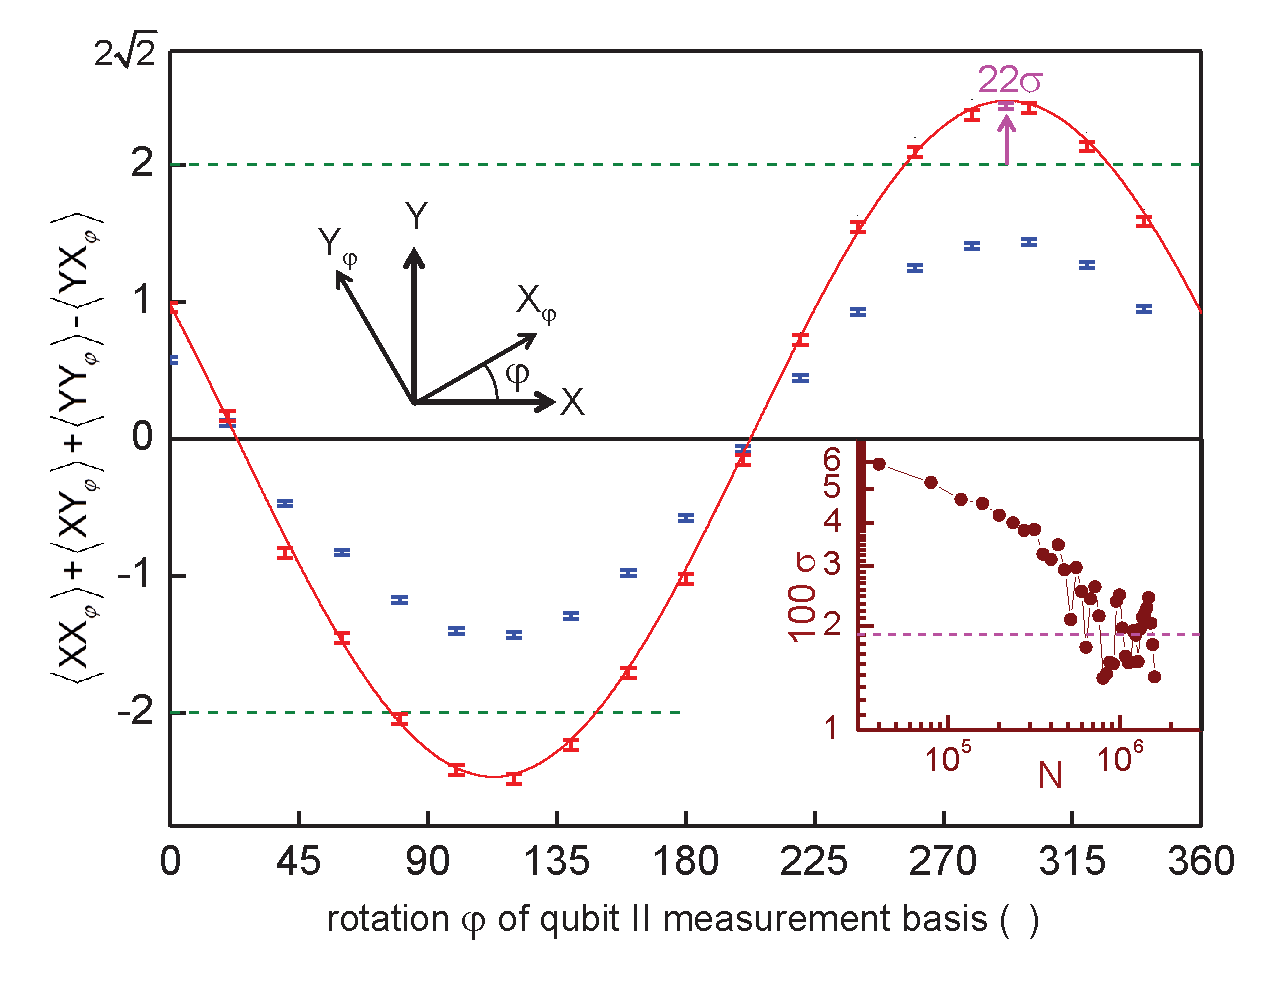
\includegraphics[width=0.8\textwidth]{./material/papers/iswap/figures/chsh}
	\end{tabular}
	\caption[]{a) Experimental pulse sequence used in the CHSH experiment. It consists in exciting one of the qubits to the state $\ket{1}$, bringing it in resonance with the other qubit for a well-defined duration, performing single-qubit rotations to align the qubit state with the desired measurement basis and finally measuring the $\bracket{\hat{\sigma}_z^I\cdot\hat{\sigma}_z^{II}}$ operator of the two-qubit register. b) Expectation value of the $\bracket{\mathrm{CHSH}}$ operator measured for an ensemble of identically prepared Bell states $1/\sqrt{2}(\ket{01}+e^{-i\phi}\ket{10})$, plotted as a function of the rotation $\varphi$ of the measurement basis. Blue markers correspond to measurement data uncorrected for readout errors, red markers to corrected data. The solid line represents the best fit to the theory. The inset shows the standard deviation $\sigma$ of the maximum value of the $\bracket{\mathrm{CHSH}}$ operator as a function of the sample size. For large sample sizes, $\sigma$ is limited by experimental drift of the measurement basis.}
	\label{fig:chsh}
	\label{fig:chsh_pulse_sequence}
\end{figure}

\subsubsection{Errors} 

Besides obvious readout errors, the main source of errors in our experiment is drift of the measurement equipment. Most importantly, the phase of the arbitrary waveform generator (AWG), which generates the sideband pulses for driving the qubits, can drift with respect to the phases of the microwave sources, thereby changing the effective phase of the measurement basis of the CHSH operator. Fig. \ref{fig:chsh_drift} illustrates the effect of this drift on the phase of the generated Bell state. Shown is the phase of the state $\ket{\phi}$ as in eq. (\ref{eq:chsh_state}) extracted from a full CHSH data set as shown in fig. \ref{fig:chsh}. When repeatedly measuring $\phi$ over a long time period, oscillations with an amplitude of $\approx 40^\circ$ can be observed. This drift can be explained by a time shift of the AWG of the order of $200\;\mathrm{ps}$, which has indeed been observed independently using a fast oscilloscope. In order to minimize the drift during a single Bell experiment, we perform the measurement at a time corresponding to one of the minima of the observed phase oscillation, where the drift is smallest.

\begin{SCfigure}[1.0][hb!]
	\centering
	\includegraphics[width=9cm]{"./data/ct5/2011_03_17 - chsh/chsh_drift"}
	\caption[]{Measured phase $\phi$ of an experimentally prepared Bell state as a function of time. The phase exhibits ``oscillatory'' drift of the order of $\approx 40^\circ$ being caused by a time drift in respect to the AWG.}
	\label{fig:chsh_drift}
\end{SCfigure}

\section{Realizing a Universal Two-Qubit Gate}

We have demonstrated that it is possible to create highly entangled qubit states with our processor by preparing Bell states, performing quantum state tomography and violating the Bell inequality. However, to realize a universal two-qubit quantum processor, it is necessary to implement a {\it universal two-qubit gate}. Therefore, in the following sections we discuss how to realize and characterize such a gate.

\subsection{Principle}

We implement the maximally entangling $\sqrt{i\mathrm{SWAP}}$ gate by using the swapping interaction given by eq. (\ref{eq:swap_evolution_operator_main}) when letting the qubits evolve in resonance for a time $t_{\sqrt{i\mathrm{SWAP}}}=1/8g$, which, for our experimental value of $2g_{qq}/2\pi = 8.3\;\mathrm{MHz}$ corresponds to $t_{\sqrt{i\mathrm{SWAP}}}\approx 30\;\mathrm{ns}$. 

\subsection{Experimental Implementation}

Figure \ref{fig:iswap_pulse_sequence} shows the pulse sequence that we use to realize the $\sqrt{i\mathrm{SWAP}}$ gate with our processor for an exemplary input state. In the case shown, we excite the first qubit to the state $\ket{1}$, creating an input state $\ket{10}$. We then tune in resonance the two qubits for a time $t_{\sqrt{i\mathrm{SWAP}}}$. After tuning the qubits out of resonance again, we apply two single-qubit $Z$-gates to compensate the dynamical phases acquired during the swap. Then, we optionally apply single-qubit tomography gates and finally read out the qubit state at the optimal readout working point. Using this technique, we can reconstruct the density matrix of the quantum state after applying the two-qubit gate to it. Similarly, we can perform quantum state tomography on the input state to obtain its density matrix. Reconstructing the input and output density matrices for a range of different input state will then allow us to fully characterize the gate operation.

\begin{figure}[ht!]
	\centering
		\includegraphics[width=0.8\textwidth]{./material/figures/measurement/qubit_iswap_full}
	\caption{Experimental pulse sequence used for implementing the two-qubit $\sqrt{i\mathrm{SWAP}}$ gate. The sequence shown for an exemplary input state $\ket{10}$ consists in exciting the first qubit to the state $\ket{1}$, bringing the qubits in resonance for a time $t=1/8g$, separating them and compensating the acquired dynamical phases by using two single-qubit $Z$-pulses. Finally, optional tomographic pulses are applied before reading out the qubit state at the optimal readout frequencies of the qubits.}
	\label{fig:iswap_pulse_sequence}
\end{figure}


\subsection{Quantum Process Tomography of the Gate}

To characterize the fidelity of our quantum gate, we perform {\it quantum process tomography} \citep{poyatos_complete_1997}. This procedure allows us to fully characterize an experimental quantum process, such as our implementation of the $\sqrt{i\mathrm{SWAP}}$ gate. The approach that we use in this work is called {\it standard quantum process tomography} (SQPT). Note that there exist other common methods such as ancilla-assisted quantum process tomography \citep{dur_nonlocal_2001,dariano_quantum_2001,altepeter_ancilla-assisted_2003}, that we will not discuss.

\subsubsection{Theoretical Description of a Quantum Process}

As explained in section \ref{section:master_equation}, any quantum process can be described by a set of Kraus operators, as given by eq. (\ref{eq:kraus_representation}):
%
\begin{equation}
\begin{mathcal}E\end{mathcal}(\rho) = \sum\limits_i^{N_k} E_i \rho E_i^\dagger \label{eq:kraus_representation_2}
\end{equation}
%
Now, if we express these operators $E_i$ in a fixed operator basis $\tilde{E}_j$ such that $E_i = \sum_j a_{ij} \tilde{E}_{j}$, we can rewrite eq. (\ref{eq:kraus_representation_2}) as

\begin{eqnarray}
 \mathcal{E}(\rho) & = & \sum\limits_i \sum\limits_j^{4^n} a_{ij} \tilde{E}_j \;\rho\; \sum\limits_k^{4^n} a_{ik}^* \tilde{E}_k^\dagger \\
& = & \sum\limits_{j,k}^{4^n}\tilde{E}_j \; \rho \; \tilde{E}_k^\dagger \sum\limits_i a_{ij} a_{ik}^* \\
& = & \sum\limits_{j,k}^{4^n}\tilde{E}_j \; \rho \; \tilde{E}_k^\dagger \; \chi_{jk}, \label{eq:process_chi_representation}
\end{eqnarray}
where we defined $\chi_{jk} = \sum\limits_i a_{ij} a_{ik}^*$. This is the $\chi$-matrix representation of the quantum process in the basis $\{\tilde{E}_i\}$. In this representation, all the information on the process is contained in the matrix $\chi$.

\subsubsection{Implementation}

The goal of QPT is to obtain the coefficients of the $\chi$-matrix -- or any other complete parametrization of the process -- from a set of experimentally measured input density matrices $\{\rho_i\}$ and output matrices $\{\mathcal{E}(\rho_i)\}$. We can fully characterize a quantum process acting on an $n$-dimensional Hilbert space by measuring $2\otimes 4^n$ experimental density matrices (or $4^n$ when assuming that no errors occur during the preparation of the input states, which thereby are known), corresponding to $\otimes 4^{2n}$ measured parameters, which equals the number of free parameters of a $n$-qubit $\chi$ matrix. We implement QPT for a n-qubit system by using the following procedure:

\begin{enumerate}
\item Choose a set of operators $\tilde{E}_i$ that forms a full basis operators acting on the given Hilbert space. For n-qubit process tomography we usually choose $\tilde{E}_{i_1,i_2 \hdots i_n} = \hat{\sigma}_{i_1}\otimes \hat{\sigma}_{i_2}\hdots\otimes\hat{\sigma}_{i_n}$, where $\hat{\sigma}_i$ are the single-qubit Pauli operators and $i\in\{I,X,Y,Z\}$. For a Hilbert space of dimension $n$, this yields $4^n$ operators (including the trivial operator $I^{\otimes n}$).
\item Choose $4^n$ pure quantum states $\ket{\phi_i}$ such that the basis $\{\ket{\phi_1}\bra{\phi_1}$, $\ket{\phi_1}\bra{\phi_2}\hdots$, $\ket{\phi_{4^n}}\bra{\phi_{4^n-1}},\ket{\phi_{4^n}}\bra{\phi_{4^n}}\}$ spans the whole Hilbert space of input density matrices $\rho$. Usually, for a n-qubit system we choose $\ket{\phi} \in \{\ket{0},\ket{1},(\ket{0}+\ket{1})/\sqrt{2},(\ket{0}+i\ket{1})/\sqrt{2}\}^{\otimes n}$, where $^{\otimes n}$ denotes the n-dimensional Kronecker product of all possible permutations.
\item Prepare each of the chosen input states $\rho_i = \ket{\phi_i}\bra{\phi_i}$, apply the gate operation and determine the output states $\mathcal{E}(\ket{\phi_i}\bra{\phi_i})$ by quantum state tomography. Optionally, perform quantum state tomography of the prepared state $\rho_i$ as well to determine experimental preparation and tomography errors.
\end{enumerate}

After having determined the $\rho_i$ and $\mathcal{E}(\rho_i)$, we obtain the $\chi$-matrix by the following procedure: First, we write $\mathcal{E}(\rho_i) = \sum_j \lambda_{ij} \tilde{\rho}_j$, in a complete basis $\{\tilde{\rho}_1,\hdots,\tilde{\rho}_{2^n}\}$ for $2^n$x$2^n$ matrices (usually we choose matrices with elements $(\tilde{\rho}_i)_{ab}=\delta_a^i\delta_b^j$, where $i$ and $j$ run over all column and row indices). Writing $\tilde{E}_m \tilde{\rho}_j \tilde{E}_n^\dagger = \sum_k \beta_{jk}^{mn}\tilde{\rho}_k$, with a $4^n\otimes 4^n \otimes 4^n \otimes 4^n$ tensor $\beta_{jk}^{mn}$, we can insert this into eq. (\ref{eq:process_chi_representation}) and obtain
%
\begin{eqnarray}
\sum\limits_k \lambda_{ik} \tilde{\rho}_k & = & \sum\limits_{m,n} \chi_{mn} \sum\limits_k \beta_{ik}^{mn} \tilde{\rho}_k  
\end{eqnarray}
%
Equating the two sides yields $\lambda_{ik} = \sum_{m,n}\beta_{ik}^{mn}\; \chi_{mn}$, which, by linear inversion,  gives $\chi$.

\smallskip

Similar to quantum state tomography, experimental errors occurring during quantum process tomography can produce a process matrix $\chi$ that is {\it non-physical} in the sense that the resulting quantum process does not obey the three axioms stated in section \ref{section:master_equation}. Therefore, we render the obtained $\chi$ matrix physical by numerically searching the  physical process matrix $\chi_{ph}$ that has the smallest distance to the original one $d=\|\chi-\chi_{ph}\|$, using e.g. the Hilbert-Schmidt norm $\|A\|_{HS} = \mathrm{Tr}(|A|)^2$. 

\subsubsection{The Kraus Representation of the Process}

To go back from the $\chi$-matrix representation of the quantum process to the Kraus form given by eq. (\ref{eq:kraus_representation}), we write each process-independent operator $\tilde{E}_i$ as a sum of all the Kraus operators $E_l$, such that
%
\begin{equation}
	\tilde{E}_i = \sum\limits_l a_{il}\; E_l
\end{equation}
%
Inserting this into eq. (\ref{eq:process_chi_representation}), we obtain
%
\begin{eqnarray}
\begin{mathcal}E\end{mathcal}(\rho) & = & \sum\limits_{j,k}\chi_{jk}\sum\limits_{l,m} a_{jl}a_{km}^* E_l \rho E_m^\dagger   \label{eq:process_chi_transformed} \\
& = & \sum\limits_i E_i \rho E^\dagger_i
\end{eqnarray}
%
We find hence the condition $\sum\limits_{j,k} \chi_{jk}a_{jl}a_{km}^* = \delta_l^m$, or, written in matrix form $A\chi A^\dagger = \mathrm{I}$, which is fulfilled if $A$ is the matrix of eigenvectors of $\chi$, multiplied by the square root of the corresponding matrix of eigenvalues. It is thus easy to obtain the Kraus representation of the quantum process by diagonalizing the Hermitian matrix $\chi$.

\smallskip

The Kraus operator form of the quantum process is useful since it allows us to easily visualize the different operators acting on the density matrix $\rho$. By ordering the Kraus operators as a function of their associated eigenvalues, one obtains the different unitary and non-unitary processes acting together on the density matrix $\rho$, ordered by importance.


\subsubsection{Unitary and Non-Unitary Gate Errors}

\begin{SCfigure}[1.0][ht!]
	\centering
	\includegraphics[width=0.4\textwidth]{./material/figures/2-qubit-processor/swap_energy_levels}
	\caption{Energy level diagram illustrating the possible swapping interactions of two three-level Transmon qubits. Resonant transitions are a)  the $\ket{01}\leftrightarrow\ket{10}$ and $\ket{12}\leftrightarrow\ket{21}$ transitions at $\omega_{01}^I = \omega_{01}^{II}$ (with swapping frequencies $g_{qq}$ and $2g_{qq}$, respectively), b) the $\ket{11}\leftrightarrow\ket{20}$ transition at $\omega_{12}^{I} = \omega_{01}^{II}$ and c) the $\ket{11}\leftrightarrow\ket{02}$ transition at $\omega_{01}^I = \omega_{12}^{II}$ (both with a swapping frequency $\sqrt{2}g_{qq}$).}
	\label{fig:swap_energy_levels}
\end{SCfigure}

After having eliminated the tomography errors, only gate errors remain. These can be unitary or non-unitary errors occurring during the quantum process. We estimate both of these errors by fitting the experimental $\chi$ matrix to a master equation model of the quantum process which includes unitary (a frequency offset when performing the swapping interaction and phase errors in the compensating $Z$ pulses applied after the swap) and non-unitary error operators (qubit relaxation and dephasing during the whole process). Typically, the relaxation and dephasing rates employed in the simulation are chosen in accordance with experimentally measured $T_1$ times and a phenomenological $T_2$ time, as discussed in section \ref{section:creation_of_entanglement}. The unitary error parameters are used as fitting parameters to maximize the fidelity between the experimentally measured process matrix $\chi$ and the simulated one $\chi_{sim}$. Using this technique, we can calculate an error budget of the quantum process that quantifies the contributions of individual error sources. 

\smallskip

\begin{figure}[ht!]
	\centering
	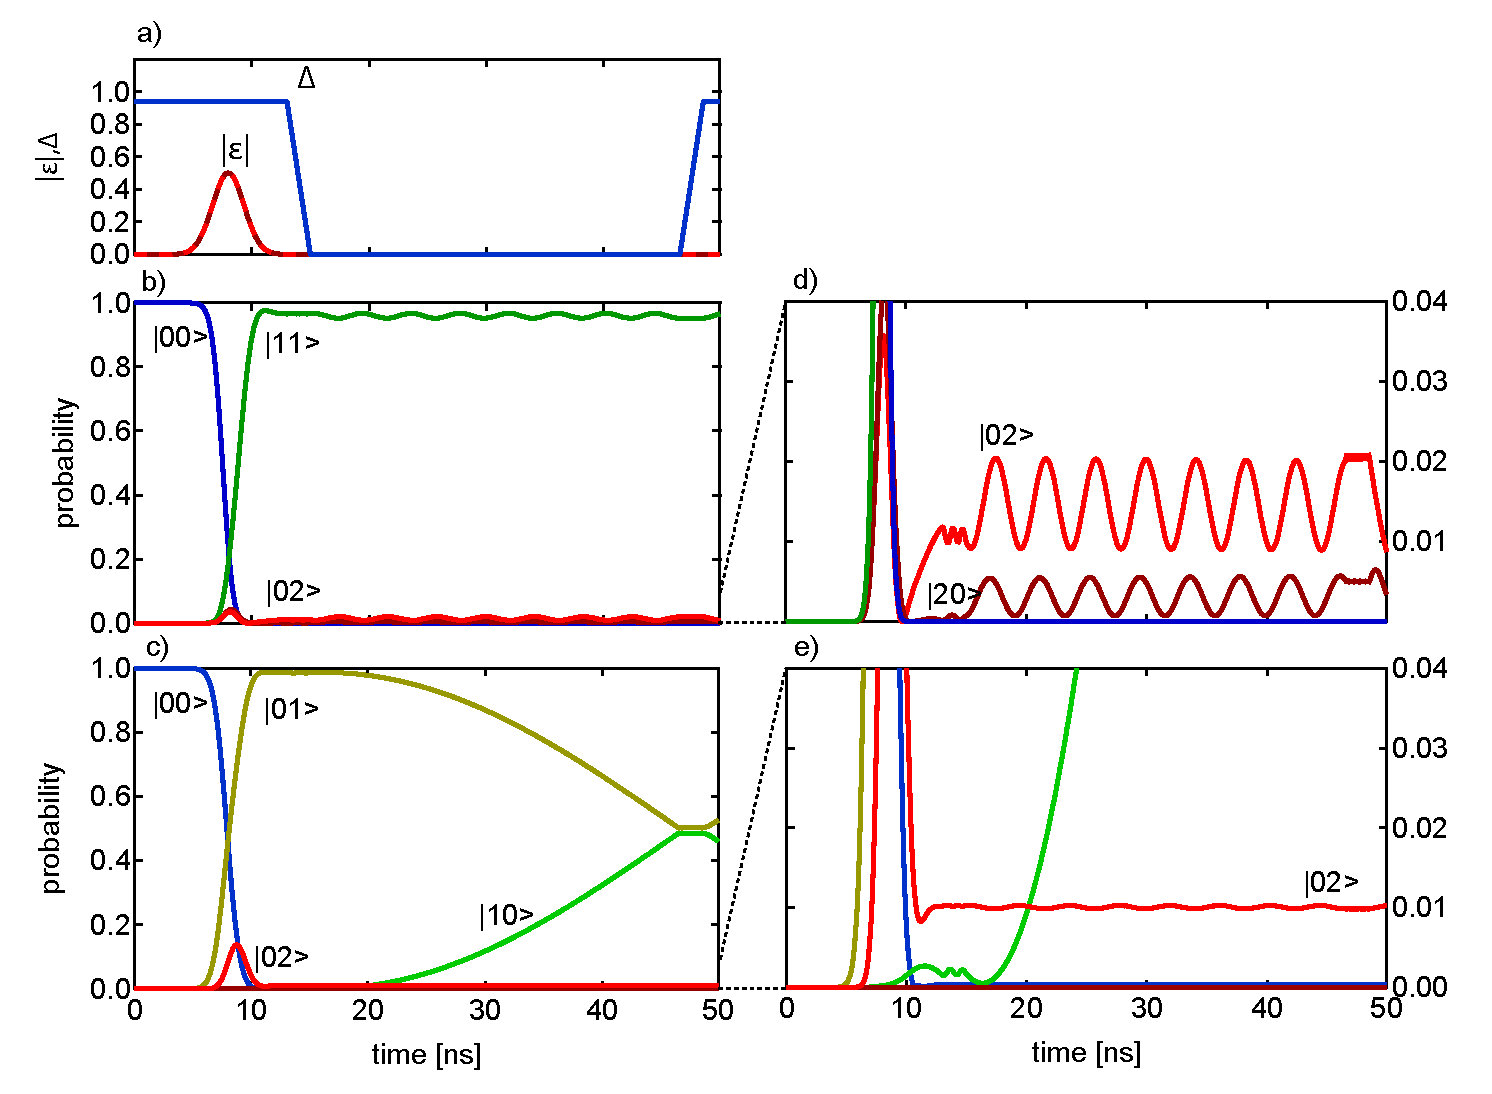
\includegraphics[width=\textwidth]{./data/simulation/three_level_swap/plots}
	\caption{a1) Drive and flux waveforms for a simulated $i\sqrt{\mathrm{SWAP}}$ gate between two three-level Transmons. a2/a3) State occupation probabilities during the simulation for the input states $\ket{01}$ (a2) and $\ket{11}$ (a3). b1/b2) show a zoom-in on the two figures a2/a3). In both cases, a small excitation of the higher Transmon level $\ket{2}$ can be observed in the simulation. For the $\ket{11}$ input state, an oscillation between the states $\ket{11}$ and $\ket{02}$/$\ket{20}$ can be observed, which is an unwanted effect. }
	\label{fig:swap_3_level_data}
\end{figure}

An error source that we analyze here is the leakage to the higher Transmon level $\ket{2}$, as discussed in section \ref{section:charge_driving}. This error can occur while driving the qubits or due to the swapping interaction between the $\ket{11}\leftrightarrow\ket{20}$ and $\ket{11}\leftrightarrow\ket{02}$ states of the three-level two-qubit Hamiltonian given by eq. (\ref{eq:three_level_interaction_hamiltonian}), as illustrated in fig. \ref{fig:swap_energy_levels}. To quantify the possible error rates associated with this leakage, we perform a simulation of an $i\sqrt{\mathrm{SWAP}}$ gate between two three-level Transmons, using the measured qubit parameters. The Hamiltonian used for this simulation are explained in detail in section \ref{section:three_level_simulation}. Just as in our experiment, in the simulation we generate 16 different input states (the same ones as used above for the QPT) using simulated Gaussian drive pulses with a rise time of $\delta t = 4\;\mathrm{ns}$ while the qubits are detuned by $\Delta_{qq}/2\pi = 150\;\mathrm{MHz}$. We then reduce the detuning to $\Delta_{qq} = 0$ during $t_\mathrm{SWAP}\approx 31 \;\mathrm{ns}$ using a simulated flux pulse with a $2\;\mathrm{ns}$ rise time, as shown in fig. \ref{fig:swap_3_level_data}a1. We calculate then numerically the state fidelity of the output state as compared to an ideal output state that is calculated using the $\sqrt{i\mathrm{SWAP}}$ operation applied to the simulated input state. By examining the output density matrices we can then give an upper bound for the leakage error into the state $\ket{2}$, which in our case is $\approx 1.5\;\%$. Figure \ref{fig:swap_3_level_data} exemplarily shows the simulated state occupation probabilities for the two input states $\ket{01}$ and $\ket{11}$. In both cases, a small excitation of the $\ket{02}$ and $\ket{20}$ Transmon states can be observed. The $\ket{11}$ input state, which should not be affected by the SWAP operation, shows a small oscillation due to the coupling to the $\ket{02}$ state.

\smallskip

Since the obtained error rates are low, we neglect possible leakage error into the state $\ket{2}$ when performing quantum state tomography of the quantum gate in this work.

\subsubsection{Tomographic Errors} \label{section:tomographic_errors}

When analyzing experimental errors of our implementation of the $\sqrt{iSWAP}$ gate, we characterize unitary and non-unitary gate errors as well as tomography errors. The former are associated to errors in the quantum process itself, whereas the latter are caused by unitary and non-unitary errors during quantum state tomography.

\smallskip

Tomographic errors are removed from the process map of our $\sqrt{iSWAP}$
gate using the following method: The measured Pauli sets corresponding
to the sixteen prepared input states are first fitted by a model including
errors both in the preparation of the state (index $\mathrm{prep}$) and in
the tomographic pulses (index $\mathrm{tomo}$). The errors included are angular
errors $\varepsilon_{\mathrm{I,II}}^{\mathrm{prep}}$ on the nominal
$\pi$ rotations around $X_{\mathrm{I,II}}$, $\eta_{\mathrm{I,II}}^{\mathrm{prep,tomo}}$and
$\delta_{\mathrm{I,II}}^{\mathrm{prep,tomo}}$ on the nominal $\pi/2$
rotations around $X_{\mathrm{I,II}}$ and $Y_{\mathrm{I,II}}$, a
possible departure $\xi_{\mathrm{I,II}}$ from orthogonality of $\left(\overrightarrow{X_{\mathrm{I}}},\overrightarrow{Y_{\mathrm{I}}}\right)$ and $\left(\overrightarrow{X_{\mathrm{II}}},\overrightarrow{Y_{\mathrm{II}}}\right)$,
and a possible rotation $\mu_{\mathrm{I,II}}$ of the tomographic
$XY$ frame with respect to the preparation one. The rotation operators
used for preparing the states and doing their tomography are thus
given by

\[
\begin{array}{c}
X_{\mathrm{I,II}}^{\mathrm{prep}}(\pi)=e^{-\mathrm{i}\left(\pi+\varepsilon_{\mathrm{I,II}}^{\mathrm{prep}}\right)\hat{\sigma}_{\mathrm{x}}^{\mathrm{I,II}}/2},\\
X_{\mathrm{I,II}}^{\mathrm{prep}}(-\pi/2)=e^{+\mathrm{i}\left(\pi/2+\eta_{\mathrm{I,II}}^{\mathrm{prep}}\right)\hat{\sigma}_{\mathrm{x}}^{\mathrm{I,II}}/2},\\
Y_{\mathrm{I,II}}^{\mathrm{prep}}(\pi/2)=e^{-\mathrm{i}\left(\pi/2+\delta_{\mathrm{I,II}}^{\mathrm{prep}}\right)\left[\mathrm{cos}\left(\xi_{\mathrm{I,II}}\right)\hat{\sigma}_{\mathrm{y}}^{\mathrm{I,II}}\mathrm{-sin}\left(\xi_{\mathrm{I,II}}\right)\hat{\sigma}_{\mathrm{x}}^{\mathrm{I,II}}\right]/2},\\
X_{\mathrm{I,II}}^{\mathrm{tomo}}(\pi/2)=e^{-\mathrm{i}\left(\pi/2+\eta_{\mathrm{I,II}}^{\mathrm{tomo}}\right)\left[\mathrm{\mathrm{sin}\left(\mu_{I,II}\right)\hat{\sigma}_{x}^{I,II}+cos}\left(\mu_{\mathrm{I,II}}\right)\hat{\sigma}_{\mathrm{y}}^{\mathrm{I,II}}\right]/2},\\
Y_{\mathrm{I,II}}^{\mathrm{tomo}}(-\pi/2)=e^{+\mathrm{i}\left(\pi/2+\delta_{\mathrm{I,II}}^{\mathrm{tomo}}\right)\left[\mathrm{cos}\left(\mu_{\mathrm{I,II}}+\xi_{\mathrm{I,II}}\right)\hat{\sigma}_{\mathrm{y}}^{\mathrm{I,II}}\mathrm{-sin}\left(\mu_{\mathrm{I,II}}+\xi_{\mathrm{I,II}}\right)\hat{\sigma}_{x}^{\mathrm{I,II}}\right]/2}.\end{array}\]
The sixteen prepared input states are then $\{ \rho_{\mathrm{in}}^{\mathrm{e}}=U\left|0\right\rangle \left\langle 0\right|U^{\dagger}\} $
with 
%
\begin{equation}
\{ U\} =\{I_{\mathrm{I}}, X_{\mathrm{I}}^{\mathrm{prep}}(\pi), Y_{\mathrm{I}}^{\mathrm{prep}}(\pi/2),X_{\mathrm{I}}^{\mathrm{prep}}(-\pi/2)\}\otimes\{I_{\mathrm{II}},X_{\mathrm{II}}^{\mathrm{prep}}(\pi),Y_{\mathrm{II}}^{\mathrm{prep}}(\pi/2),X_{\mathrm{II}}^{\mathrm{prep}}(-\pi/2)\},
\end{equation}
%
and each input state yields a Pauli set $\left\{ \left\langle P_{\mathrm{k}}^{\mathrm{e}}\right\rangle =Tr\left(\rho_{\mathrm{in}}^{\mathrm{e}}P_{\mathrm{k}}^{\mathrm{e}}\right)\right\} $
with $\left\{ P_{\mathrm{k}}^{\mathrm{e}}\right\} =\{I_{\mathrm{I}},X_{\mathrm{I}}^{\mathrm{e}},Y_{\mathrm{I}}^{\mathrm{e}},Z_{\mathrm{I}}\}\otimes\{I_{\mathrm{II}},X_{\mathrm{II}}^{\mathrm{e}},Y_{\mathrm{II}}^{\mathrm{e}},Z_{\mathrm{II}}\}$,
$X^{\mathrm{e}}=Y^{\mathrm{tomo}}(-\pi/2)^{\dagger}\hat{\sigma}_{z}Y^{\mathrm{tomo}}(-\pi/2)$,
and $Y^{\mathrm{e}}=X^{\mathrm{tomo}}(\pi/2)^{\dagger}\hat{\sigma}_{\mathrm{z}}X^{\mathrm{tomo}}(\pi/2)$.

Knowing the tomographic errors and thus $\left\{ \left\langle P_{\mathrm{k}}^{\mathrm{e}}\right\rangle \right\} $,
we then invert the linear relation $\left\{ \left\langle P_{\mathrm{k}}^{\mathrm{e}}\right\rangle =Tr\left(\rho P_{\mathrm{k}}^{\mathrm{e}}\right)\right\} $
to find the $16\times16$ matrix $B$ that links the vector $\overrightarrow{\left\langle P_{\mathrm{k}}^{\mathrm{e}}\right\rangle }$
to the columnized density matrix $\overrightarrow{\rho}$, i.e. $\overrightarrow{\rho}=B.\overrightarrow{\left\langle P_{\mathrm{k}}^{\mathrm{e}}\right\rangle }$.
The matrix $B$ is finally applied to the measured sixteen input and
sixteen output Pauli sets to find the sixteen $(\rho_{\mathrm{in},},\rho_{\mathrm{out}})_{\mathrm{k}}$
couples to be used for calculating the gate map.

\smallskip

For our data, the best fit to the modeled $\left\{ \left\langle P_{k}^{e}\right\rangle \right\} $
set to the measured input Pauli sets yields $\varepsilon_{\mathrm{I}}^{\mathrm{prep}}=-1\text{\textdegree}$,
$\varepsilon_{\mathrm{II}}^{\mathrm{prep}}=-3\text{\textdegree}$,
$\eta_{\mathrm{I}}^{\mathrm{prep}}=3\text{\textdegree}$, $\mathrm{\eta}_{\mathrm{II}}^{\mathrm{prep}}=4\text{\textdegree}$,
$\delta_{\mathrm{I}}^{\mathrm{prep}}=-6\text{\textdegree}$, $\delta_{\mathrm{II}}^{\mathrm{prep}}=-3\text{\textdegree}$,
$\eta_{\mathrm{I}}^{\mathrm{tomo}}=-6\text{\textdegree}$, $\eta_{\mathrm{II}}^{\mathrm{tomo}}=-4\text{\textdegree}$,
$\lambda_{\mathrm{I}}^{t\mathrm{omo}}=12\text{\textdegree}$, $\lambda_{\mathrm{II}}^{\mathrm{tomo}}=5\text{\textdegree}$,
$\xi_{\mathrm{I}}=1\text{\textdegree}$, $\xi_{\mathrm{II}}=-2\text{\textdegree}$,
and $\mu_{\mathrm{I}}=\mu_{\mathrm{II}}=-11\text{\textdegree}$. More details can be found in appendix \ref{chapter:papers}.


\begin{figure}[p]
	\centering
		\includegraphics[width=1.0\textwidth]{"./data/ct5/2011_04_21 - grover and tomo/good_data/process -matrices 1"}
	\caption{The experimental input-output density matrices of the quantum process tomography of the $\sqrt{i\mathrm{SWAP}}$ gate. Shown are the measured density matrices of 16 different input states and the corresponding output matrices with their state fidelities. The ideal matrices are overlaid in black. (part I/II)}
	\label{fig:process_matrices_1}
\end{figure}

\begin{figure}[p]
	\centering
		\includegraphics[width=1\textwidth]{"./data/ct5/2011_04_21 - grover and tomo/good_data/process -matrices 2"}
	\caption{}
	\label{fig:process_matrices_2}
\end{figure}

\subsection{Experimental Results}

\begin{figure}[ht!]
	\centering
		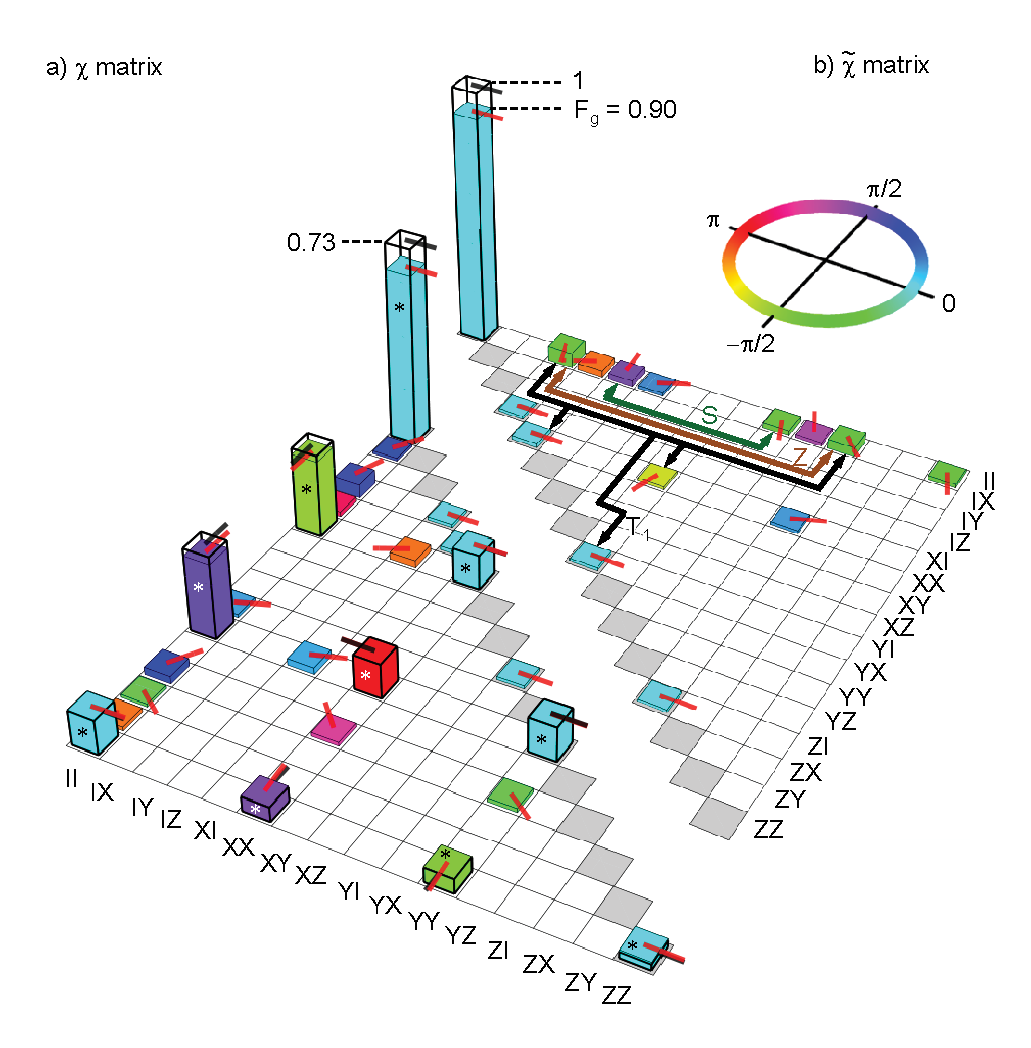
\includegraphics[width=1.\textwidth]{./material/papers/iswap/figures/chi_matrix_and_error_process}
	\caption{Reconstructed $\chi$ process matrix of our implementation of the $\sqrt{i\mathrm{SWAP}}$ quantum gate. a) Lower half of the Hermitian $\chi$ matrix. b) Error process $\tilde{\chi}=\chi\cdot\chi_{id}^{-1}$ of the measured $\chi$ matrix and the ideal process matrix $\chi_{id}$. The colored arrows grouping different elements of $\tilde{\chi}$ indicate unitary and non-unitary error processes to which the corresponding matrix elements can be associated.}
	\label{fig:chi_matrix_and_errors}
\end{figure}

We perform standard process tomography of our two-qubit gate by following the procedure outlined in the last sections. Figs. \ref{fig:process_matrices_1} and \ref{fig:process_matrices_2} summarize the experimentally determined input-output density matrices, measured for our two-qubit $\sqrt{i\mathrm{SWAP}}$ quantum gate. We show pairs of corresponding input and output states together, with both the reconstructed experimental density matrices as well as the ideal ones. The targeted input states are annotated below the corresponding density matrices. Above each matrix we show the trace fidelity between it and the ideal quantum state. A total of 16 input/output pairs has been measured, corresponding to a complete set of states necessary to characterize the quantum process of our gate operation.

\smallskip

From the input/output matrices, we calculate the $\chi$ matrix of the quantum process by the method described above. The resulting matrix is shown in fig. \ref{fig:chi_matrix_and_errors}. There, we show the experimentally obtained $\chi$ matrix of our $\sqrt{i\mathrm{SWAP}}$ gate as well as the error process defined as $\tilde{\chi} = \chi\cdot\chi_{id}^{-1}$, where $\chi_{id}$ corresponds to the ideal gate process. $\chi_{id}$ is also shown as black outlines overlaid to the measured $\chi$ matrix. The arrows connecting different parts of the $\tilde{\chi}$ matrix group several unitary and non-unitary error processes that can be attributed to the observed elements.

\smallskip

\begin{figure}[ht!]
	\centering
		\includegraphics[width=1.\textwidth]{"./data/ct5/2011_04_21 - grover and tomo/good_data/process_kraus_operators"}
	\caption{The Kraus operators of the experimental process matrix $\chi$, as shown in fig. \ref{fig:chi_matrix_and_errors}a. Shown are only the four operators with the largest eigenvalues, which together sum up to $>0.999$ and therefore describe the physical process with high accuracy.}
	\label{fig:kraus_operators}
\end{figure}

From the experimental $\chi$ matrix, we calculate the Kraus operators of the corresponding quantum process. In our case, the four largest eigenvalues $\lambda_i$ of $\chi$ (for which $\sum\limits_i \lambda_i = 1$) sum up to a value $>0.999$ and therefore suffice to describe the process with high accuracy. The corresponding four Kraus operators are shown in fig. \ref{fig:kraus_operators}. As can be seen, the operator associated to the largest eigenvalue $\lambda=0.909$ corresponds closely to a unitary $\sqrt{i\mathrm{SWAP}}$ operator. The other operators are largely non-unitary and describe the decoherence in the quantum process.

\subsection{Gate Error Analysis}

We find a total gate error of $10 \%$, where we can attribute $8\%$ of the errors to relaxation and decoherence during the process and $2\%$ to unitary gate errors.

\section{Conclusion}

In this chapter we demonstrated that we can implement a universal set of quantum gates on our two-qubit processor. We created and characterized entangled two-qubit states, performed quantum state tomography, implemented the $\sqrt{iSWAP}$ quantum gate with a fidelity of $90\%$ and analyzed the most important error sources of the gate operation.

\smallskip

In the next chapter, we use the set of universal gates to run a simple quantum search algorithm on our two-qubit processor, showing that we are able to demonstrate quantum speed-up for a real-world problem, albeit at a scale which is not yet practically useful.